\documentclass[a4paper,oneside,frenchb,10pt]{article}

\usepackage[T1]{fontenc}
\usepackage[utf8x]{inputenc}
\usepackage{amsmath}
\usepackage{babel}
\usepackage{babel}
\usepackage{fancyhdr}
\usepackage{fourier}
\usepackage{fullpage}
\usepackage{graphicx}
\usepackage{hyperref}
\usepackage{listings}
\usepackage{multicol, float} % Use float to include figures in multicols.
\usepackage{textcomp}
\usepackage{url}

\hypersetup{colorlinks=true, linkcolor=black}


\setlength{\headheight}{15.2pt}
\setlength{\headsep}{10pt}

\pagestyle{fancy}

\fancyhf{}

\lhead{\fancyplain{}{Manuel Utilisateur}}
\rhead{\fancyplain{}{\thepage}}

\setlength{\parindent}{0pt}
\setlength{\parskip}{4pt plus 2pt minus 1pt}
\setcounter{secnumdepth}{0}

\title{Manuel Utilisateur}
\author{\emph{The BackSynth Boys}}

\begin{document}

\thispagestyle{empty}

\begin{center}
\huge Manuel Utilisateur
\end{center}

\vspace{1cm}

\tableofcontents

\section{Introduction}

Tout d'abord, nous vous remercions d'avoir choisi notre logiciel
\textbf{SynthPro}. Les \emph{BackSynth Boys} ont travaillé dur pour produire ce logiciel
sonore qui saura vous convaincre par sa haute qualité.

\section{Présentation générale}

\textbf{SynthPro} est un logiciel de synthèse sonore dont le but est de 
simuler les différents modules utilisés par les synthétiseurs analogiques
dits à synthèse soustractive.

Ce logiciel est entièrement modulaire. Vous pouvez placer les modules
mis à votre disposition, les lier entre eux et entendre le résultat du
montage en temps-réel. Il ne reste plus qu'à laisser votre créativité
faire le reste.

\section{Utilisation du logiciel}

Lorsque vous lancez le logiciel, vous voyez apparaitre son interface~:

\begin{itemize}
\item
  Les menus et la barre d'outils en haut~;
\item
  Les modules disponibles classés selon leur type, à gauche~;
\item
  Un grand espace vide que vous allez pouvoir remplir~!
\end{itemize}
\subsection{Les menus}

Ils sont composés de deux sous-menus~: \emph{File} et \emph{Help}, chacun 
possédant plusieurs sous-items.

\paragraph{File}
\begin{description}
\item[\emph{New}]
  Vous permet de recommencer un nouveau montage, après
  confirmation de votre part d'effacer le montage courant.
\item[\emph{Open}]
  Vous permet de charger un montage que vous auriez au préalable
  sauvegardé.
\item[\emph{Save}]
  Utilisez cette option pour sauvegarder votre montage dans le
  fichier désiré. Vous pourrez ainsi le relire plus tard devant vos
  amis, épatés.
\item[\emph{Play/Pause}]
  Permet de stopper ou de relancer la lecture du montage.
  Stopper la lecture revient à couper le son et stopper toute la gestion
  des modules en temps-réel.
\item[\emph{Exit}]
  Provoque la sortie de l'application.
\end{description}

\paragraph{Help}
\begin{description}
\item[\emph{About}]
  Donne des informations relatives au logiciel et ses
  développeurs.
\item[\emph{About Qt}]
  Donne des informations relatives au \emph{framework} utilisé pour
  le développement de ce logiciel.
\end{description}

\subsection{La barre d'outils}

Les cinq actions disponibles dans la barre d'outils sont identiques à ce
que l'on peut trouver dans le menu \emph{File}, ci-dessus~: \emph{New}, \emph{Load}, \emph{Save},
\emph{Exit}, et \emph{Play/Pause}.

\subsection{Les modules}

Les modules sont classés en trois catégories~:

\begin{itemize}
\item
  Les modules d'entrée (\emph{Input modules})~;
\item
  Les modules de traitement (\emph{Modules})~;
\item
  Les modules de sortie (\emph{Output modules}).
\end{itemize}

Les modules d'entrée représentent les modules qui peuvent créer des
signaux à partir de rien. Ce sont les composants de base d'un montage et
ne disposent pas de ports d'entrée.

Les modules de traitement sont intermédiaires~: ils prennent un signal,
le modifient et l’envoient sur leur sortie.

Enfin, les modules de sortie sont mis en fin de chaîne~: ils acceptent
une entrée, mais ne renvoient rien car ils n'ont pas de sortie.

L'interface vous sera présentée ultérieurement.

\section{Présentation générale de la modularité}

\textbf{SynthPro} est un logiciel modulaire~: chaque module est une «~brique~»
qu'il est possible de placer un nombre infini de fois sur l'interface,
afin de construire votre propre montage sonore.

Un module dispose de plusieurs caractéristiques~:

\begin{itemize}
\item
  Une fonction~;
\item
  Éventuellement des ports d'entrée~;
\item
  Éventuellement des ports de sortie~;
\item
  Des paramètres.
\end{itemize}
La fonction du module est en général clairement définie par son nom.
Ainsi, le module filtre va\ldots{} filtrer ce qu'on lui donne.

Les ports d'entrée servent à fournir un signal au module. Ainsi, un
filtre aura forcément une entrée, car il a besoin de données à traiter
sur lesquelles accomplir sa fonction.

Les ports de sortie servent à renvoyer le travail produit à un autre
module, ou plus précisément, à l'une de ses entrées. Ainsi, une chaîne
entière sonore peut être fabriquée en liant les sorties des modules aux
entrées des autres.

Les paramètres des modules peuvent apparaître sous plusieurs formes~:
potentiomètres ou \emph{slider} à coulisser. Ces paramètres dépendent
entièrement du module. Ainsi, un module Mixer pourra changer le volume
de chacune de ses entrées grâce au paramètre Gain qui leur est attribué.

Les modules peuvent être reliés par des câbles virtuels, qui
représenteraient des cables électriques dans le monde «~réel~»\ldots{}
Mais les nôtres sont infaillibles.

\section{Utilisation pratique du logiciel}

\subsection{Un premier montage}

Il est maintenant temps de commencer à créer des montages sonores dignes
de ce nom. Le grand espace vide à droite de la liste des modules va
servir à cela. La première étape consiste à prendre un module et le
placer dans la zone de montage. Pour cela, cliquez sur le module désiré
grâce au bouton gauche de la souris et, sans le relâcher, déplacer votre
curseur au milieu de la zone de montage. Relâchez le bouton. Le module
va alors être créé.

Essayez de le faire avec le module d'entrée VCO, dont la fonction est de
générer des ondes sonores. Par défaut il produit une onde à 261 Hz, soit
un DO de l'octave 4. Cette valeur est inscrite au dessus du
potentiomètre \verb!K!.

Mais pour l'instant, aucun son n'est entendu. Pour cela, il faut une
sortie son~: placez à droite du module présent un module Speaker.
Celui-ci est un module de sortie~: il n'a pas de sorties, mais une
entrée. Il faut donc relier celle-ci à la sortie du VCO. Pour cela,
cliquez simplement sur l'entrée et, sans relâcher le bouton gauche de la
souris, déplacer votre curseur vers la sortie du VCO. Un câble vient
d'apparaitre. Vous pouvez voir les ports sur lesquels vous pouvez
accrocher le câble devenir verts. Les emplacements non accessibles sont
affichés en rouge. Lâchez alors le bouton pour créer la connexion entre
les deux ports. Le son produit par le VCO est maintenant reproduit par
vos haut-parleurs~!

Il vous est possible de relier tout port de sortie vers une entrée, et
inversement. Pour débrancher un câble, cliquez sur une de ses extrémités
et relâchez le bouton de la souris lorsque le câble survole une zone
non-interactive, comme le fond de la zone de montage. Il est vous
également possible de rebrancher le câble sur une autre entrée si besoin
est.

Vous pouvez ainsi ajouter tous les modules que vous désirez et les
relier entre eux. Si vous souhaitez retirer des modules, cliquez
simplement sur la croix en haut à gauche de chacun d'eux.

Vous avez maintenant toutes les clefs en main pour obtenir des sons
prodigieux~!

\subsection{Quelques précisions sur les Gate}

Comme vous avez pu le constater, certains modules disposent d'entrées
appelées \verb!Gate in!, et des sorties \verb!Gate out!. Elles se
comportent comme des entrées et sorties conventionnelles, dans le sens
où vous pourrez brancher une \verb!Gate out! à n'importe quelle entrée,
et n'importe quelle sortie à une \verb!Gate in!.

Qu'est-ce qu'une \verb!Gate!~? Il s'agit d'une entrée ou sortie un peu
spéciale, qui ne va produire ou interpréter que des fronts montant ou
descendant. Cela permet notamment au module Keyboard d'indiquer quand
une touche est pressée (front montant dans la \verb!Gate out!), ou quand
elle est relâchée (front descendant dans la \verb!Gate out!). Branchez
la \verb!Gate out! dans la \verb!Gate In! de l'ADSR, et jouez avec le
clavier~: l'onde de l'ADSR est déclenchée à chaque pression de touche~!

Remarquez également que lorsque vous créez un câble partant d'une sortie
conventionnelle, les \verb!Gates In! deviennent bleues. Cela indique que
l'utilisation de ces entrées n'est en général pas adaptée à votre
sortie, mais l'action reste cependant possible.

\section{Description des modules}

Nous allons maintenant vous présenter l'intégralité des modules que vous
pourrez utiliser.

\subsection{VCO}

\begin{multicols}{2}
\begin{figure}[H]
\centering
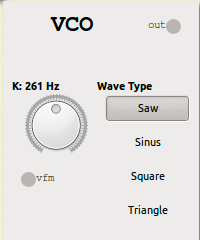
\includegraphics[width=3.5cm]{../img/png/vco.png}
\caption{VCO}
\end{figure}

Un VCO (Voltage Controlled Oscillator) permet de générer des ondes
d'amplitude définie (+5V/--5V) et de fréquence variable. Il existe
plusieurs formes d'ondes~:

\begin{itemize}
\item
  Carrée (square)~;
\item
  Dents de scie (saw)~;
\item
  Triangle~;
\item
  Sinus.
\end{itemize}

La fréquence produite par un VCO peut être définie de deux manières~:

\begin{itemize}
\item
  Par l'intermédiaire du potentiomètre \verb!K!~;
\item
  Grâce aux entrées \verb!Vfm!.
\end{itemize}
\end{multicols}

Les entrées \verb!Vfm! peuvent par exemple être connectées à un module
de type Keyboard ou LFO. Dans ce cas, les signaux d'entrées seront
additionnés avec la valeur du potentiomètre \verb!K! pour la production
de la fréquence de sortie. Si vous désirez modifier l'amplitude du
signal, il faut alors connecter le VCO à un VCA.

\subsection{VCA}

\begin{multicols}{2}
Le module VCA (Voltage Controlled Amplifier) permet d'amplifier ou
atténuer le signal passé dans l'entrée \verb!In!, vers la sortie
\verb!Out!, selon le facteur indiqué par le potentiomètre \verb!Gain!,
par défaut à 0 dB, ce qui ne modifie alors pas le signal.

La deuxième entrée, \verb!Control!, permet de faire varier dans le temps
l'amplification. Une utilisation typique est de lui connecter soit un
LFO, soit un ADSR. Notons que la tension de l'entrée Control est
additionée avec le \verb!Gain! donné par le potentiomètre.

\begin{figure}[H]
\centering
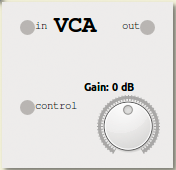
\includegraphics[width=3.5cm]{../img/png/vca.png}
\caption{VCA}
\end{figure}
\end{multicols}

\newpage

\subsection{VCF}

\begin{multicols}{2}
\begin{figure}[H]
\centering
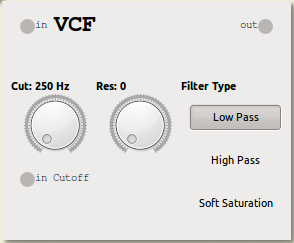
\includegraphics[width=4.5cm]{../img/png/vcf.png}
\caption{VCF}
\end{figure}

Un VCF (Voltage Controlled Filter) permet d'appliquer un filtre sur un
signal d'entrée et produire le résultat sur la sortie. Il existe
plusieurs types de filtres~:

\begin{itemize}
\item
  Filtre passe-bas (low-pass filter)~;
\item
  Filtre passe-haut (high-pass filter)~;
\item
  Saturation douce (soft saturation).
\end{itemize}

Le filtre passe-bas permet de retirer une partie des fréquences aiguës,
alors que le filtre passe-haut retire une partie des graves. La
saturation douce applique une légère saturation sur le signal d'entrée.
\end{multicols}

Le VCF dispose de deux entrées et deux potentiomètres~:

\begin{itemize}
\item
  Le potentiomètre \verb!Cutoff!~;
\item
  Le potentiomètre \verb!Resonance!~;
\item
  L'entrée \verb!In!~;
\item
  L'entrée \verb!In Cutoff!.
\end{itemize}
L'entrée \verb!In! permet en toute logique d'introduire dans le VCF le
signal sur lequel on souhaite appliquer le filtre sélectionné. Le
potentiomètre \verb!Cutoff! indique la fréquence de coupure,
c'est-à-dire la fréquence à partir de laquelle le filtre sera opérant.
Ainsi, dans le cas du filtre passe-bas, les fréquences supérieures au
\verb!Cutoff! seront atténuées. À l'inverse, le filtre passe-haut
atténuera les fréquences inférieures.

Le signal introduit dans l'entrée \verb!In Cutoff! permet également de
modifier la fréquence de coupure, qui sera additionnée à celle de
\verb!Cutoff!. Il est ainsi possible de brancher par exemple un LFO pour
obtenir des variations de fréquence de coupure dans le temps. Notons
que les facteurs de \verb!Cutoff! n'ont pas d'incidence sur le filtre de
saturation douce.

Le potentiomètre \verb!Resonance! indique, pour les filtres passe-haut
et passe-bas, le facteur d'atténuation du filtre. Plus il est faible et
plus l'atténuation est élevée. Ce facteur indique également le facteur
de saturation pour le filtre de saturation douce.

\subsection{ADSR}

\begin{multicols}{2}
\begin{figure}[H]
\centering
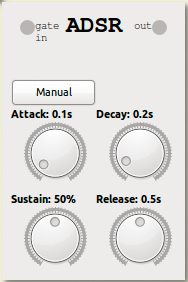
\includegraphics[width=4cm]{../img/png/adsr.png}
\caption{ADSR}
\end{figure}

Ce module permet de produire une onde dont l'intensité varie dans le
temps selon 4 paramètres, qui sont autant de potentiomètres~:

\begin{itemize}
\item
  \verb!Attack!~;
\item
  \verb!Decay!~;
\item
  \verb!Sustain!~;
\item
  \verb!Release!.
\end{itemize}

Afin de savoir quand l'onde doit commencer et s'arrêter, on utilise
l'entrée \verb!Gate In!. Un front montant dans le signal qu'elle reçoit
indique que l'onde doit commencer ou recommencer, un front descendant
qu'elle doit s'arrêter.

Lorsque l'onde est déclenchée se produit la phase d'attaque~: le signal
commence à 0~V et augmente jusqu'à atteindre 1~V. La durée de cette
évolution est donnée par le paramètre \verb!Attack!, variant de 0 à 2
secondes.
\end{multicols}

Lorsque l'attaque est terminée, vient le \verb!Decay!. Le signal diminue
progressivement jusqu'à atteindre la valeur indiquée par le
\verb!Sustain!, lui même un pourcentage de l'intensité maximum. Le
\verb!Decay! indique donc le temps en secondes entre la fin de l'attaque
(l'intensité est au maximum) et l'atteinte de l'intensité définie
par le \verb!Sustain!.

L'onde reste alors stable, jusqu'à ce que l'entrée \verb!Gate In!
reçoive un front descendant. L'onde entre alors dans sa dernière phase~:
le \verb!Release!. Le potentiomètre associé indique la durée en secondes
entre l'intensité actuelle et l'intensité à 0.

Notons qu'à tout moment peut se produire un relâchement de l'onde, selon
ce que l'entrée \verb!Gate In! reçoit. Il est cependant possible de
recommencer l'attaque alors que le \verb!Release! n'est pas encore
terminé.

Un ADSR est particulièrement adapté pour être connecté à un Keyboard
(clavier virtuel) qui va être connecté à sa \verb!Gate In!. Cela permet
ainsi de déclencher l'attaque de l'onde lorsqu'une touche du clavier
virtuel est pressée et de stopper cette onde lorsque la touche est
relâchée. Il est également utile de connecter la sortie \verb!Out! de
l'ADSR à l'entrée \verb!Control! d'un module VCA, lui même lié à un VCO
par exemple. Ainsi, presser une touche du clavier virtuel déclenchera
l'onde de l'ADSR, tandis que l'onde produite par le VCO sera amplifiée
par le VCA, dont le \verb!Gain! est paramétré par l'onde de l'ADSR.
Relire ce paragraphe plusieurs fois peut s'avérer utile si vous ne
comprenez pas.

Le bouton \verb!Manual! est utile dans le cas où vous ne voudriez pas
vous embarrasser d'un clavier virtuel pour déclencher l'onde. Presser ce
bouton déclenchera l'onde instantanément et le relâcher la fera passer
dans sa phase \verb!Release!.

\subsection{LFO}

\begin{multicols}{2}
Le LFO (Low Frequency Oscillator) vous permet de créer, à la manière
d'un VCF, une onde à une fréquence donnée. La principale différence est
que cette onde a une fréquence très faible, ce qui est particulièrement
utile pour faire évoluer un paramètre d'un module voisin.

Quatre formes d'ondes sont disponibles~:

\begin{itemize}
\item
  Carrée (square)~;
\item
  Dents de scie (saw)~;
\item
  Triangle~;
\item
  Sinus.
\end{itemize}

\begin{figure}[H]
\centering
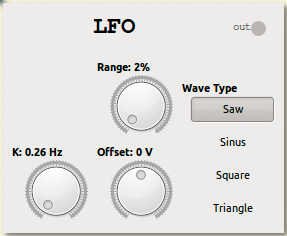
\includegraphics[width=4.5cm]{../img/png/lfo.png}
\caption{LFO}
\end{figure}
\end{multicols}

La sortie \verb!Out! peut être connectée à toute entrée d'un module dont
on veut faire varier un paramètre. Par exemple, il est très fréquent de
brancher la sortie vers l'entrée \verb!In Cutoff! d'un VCF, ce qui fera
évoluer la fréquence de coupure de son filtre. Une autre utilité est de
faire varier le \verb!Vfm! d'un VCO pour produire un effet de vibrato,
par exemple.

Trois potentiomètres peuvent être utilisés~:

\begin{itemize}
\item
  \verb!K!~;
\item
  \verb!Range!~;
\item
  \verb!Offset!.
\end{itemize}
Le paramètre \verb!K! est la fréquence produite par le LFO. Le paramètre
\verb!Range! représente l`amplitude du signal émis en sortie. Enfin,
l'\verb!Offset! ajoute une constante au signal de sortie. Cela est utile
pour centrer l'évolution de la forme d'onde choisie autour d'une
fréquence choisie, par exemple.

\newpage

\subsection{Delay}

\begin{multicols}{2}

\begin{figure}[H]
\centering
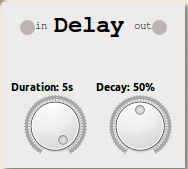
\includegraphics[width=3.5cm]{../img/png/delay.png}
\caption{Delay}
\end{figure}

Ce module permet de créer un effet de délai sur le signal d'entrée.
Ainsi, le signal émis en entrée \verb!In! sera retransmis normalement
sur la sortie \verb!Out!, mais ressortira de nouveau sur la sortie plus
tard et de manière atténuée ou non.

Ce module dispose de deux potentiomètres~:

\begin{itemize}
\item
  \verb!Duration!~;
\item
  \verb!Decay!.
\end{itemize}
\end{multicols}

Le paramètre \verb!Duration! indique la durée du retard en secondes.
\verb!Decay! est un pourcentage qui indique le facteur d'atténuation du
son reproduit après le délai \verb!Duration!. Le module reproduira le
son donné dans l'entrée \verb!In! 3 fois, atténué du facteur
\verb!Decay!, avant de le remplacer par les nouvelles données arrivant
dans l'entrée \verb!In!.

\subsection{Mixer}

\begin{multicols}{2}
Ce module permet de \emph{mixer} les différentes entrées dont il dispose.

Il permet également de régler un gain pour chacun d'entre eux. Il vous est
donc possible d'atténuer ou d'amplifier indépendamment les divers signaux entrants.

Cela peut-être particulièrement utile avant d'envoyer des données au
Speaker, car la somme de plusieurs signaux pourrait faire saturer la
sortie audio, la rendant désagréable à écouter.

\begin{figure}[H]
\centering
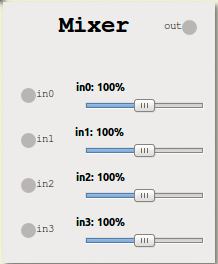
\includegraphics[width=3.5cm]{../img/png/mixer.png}
\caption{Mixer}
\end{figure}
\end{multicols}

\subsection{Sampler}

\begin{multicols}{2}
\begin{figure}[H]
\centering
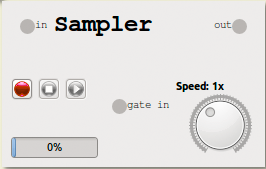
\includegraphics[width=4.5cm]{../img/png/sampler.png}
\caption{Sampler}
\end{figure}

Ce module vous permet d'enregistrer en temps-réel une petite séquence de
maximum 5 secondes et de la rejouer à volonté, à la vitesse choisie. Le
Sampler dispose d'une entrée \verb!In!, d'où provient le son à
enregistrer et une sortie \verb!Out!, d'où sortira le son produit.

Trois boutons sont disponibles~:

\begin{itemize}
\item
  \verb!Record!~;
\item
  \verb!Stop!~;
\item
  \verb!Play!.
\end{itemize}
\end{multicols}

Au début, seul le premier est disponible. Une fois l'entrée connectée,
pressez \verb!Record! pour commencer l'enregistrement. Une barre bleue
indique la progression de l'enregistrement, qui peut au maximum
atteindre 5 secondes. Pour le stopper, pressez le bouton \verb!Stop!, ou
attendez que la limite des 5 secondes soit atteinte.

Une fois qu'une séquence est enregistrée, appuyez simplement sur
\verb!Play! pour qu'elle soit produite en boucle sur la sortie
\verb!Out!. La barre de progression indique quelle partie de
l'enregistrement est actuellement jouée.

Il vous est possible à tout moment de stopper la lecture grâce au bouton
\verb!Stop!, ou enregistrer une nouvelle séquence grâce au bouton
d'enregistrement.

L'entrée \verb!Gate In! est utile pour lancer ou stopper la lecture de
l'enregistrement. Ainsi, en branchant un clavier virtuel dessus, la
pression d'une touche lancera la lecture, une nouvelle pression la
stoppera.

Enfin, un potentiomètre \verb!Speed! permet de régler la vitesse de
lecture.

\subsection{Oscilloscope}

\begin{multicols}{2}
\begin{figure}[H]
\centering
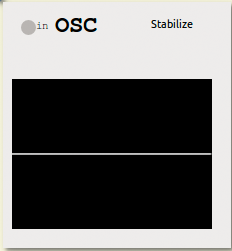
\includegraphics[width=4cm]{../img/png/oscilloscope.png}
\caption{Oscilloscope}
\end{figure}

L'oscilloscope permet de visualiser le signal qui lui est fourni en
entrée, de manière analogue à un oscilloscope réel. L'axe des abscisses
représente le temps, tandis que celui des ordonnées représente
l'amplitude du signal.

L'oscilloscope accepte des tensions allant du double de celles produites
par un VCO, soit de −10V à 10V, vous permettant de visualiser des
signaux de forte intensité.

Le bouton \verb!Stabilize! permet, comme son nom l'indique, de
stabiliser visuellement le signal d'entrée. Par défaut, cette option est
désactivée.
\end{multicols}

\subsection{Keyboard}

\begin{multicols}{2}
Ce module fait apparaître un clavier virtuel sur votre écran. Sa
principale utilité est de permettre à un VCO de produire un son à la
fréquence correspondant à la touche du clavier que vous auriez appuyée.

Il est possible d'interagir avec le clavier virtuel de deux manières~:

\begin{figure}[H]
\centering
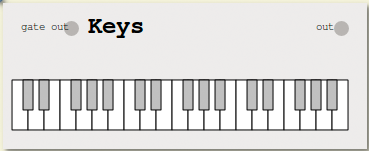
\includegraphics[width=5cm]{../img/png/keyboard.png}
\caption{Keyboard}
\end{figure}
\end{multicols}

\begin{itemize}
\item
  En cliquant sur une touche avec la souris~;
\item
  En utilisant les touches de votre clavier d'ordinateur (Q, Z, S, E, D,
  F, T, G, Y, H, U, J, K).
\end{itemize}
Il vous faudra également utiliser au moins une des deux sorties mises à
votre disposition~:

\begin{itemize}
\item
  \verb!Out!~;
\item
  \verb!Gate Out!.
\end{itemize}
La sortie \verb!Out! produit une tension relative à la fréquence émise
par le clavier. En branchant la sortie \verb!Out! sur l'entrée
\verb!Vfm! d'un VCO, il vous est ainsi possible de produire des sons à
la fréquence produite par le clavier.

La sortie \verb!Gate Out! crée une onde dont le front est montant quand
une touche du clavier virtuel est pressée, et descendant quand elle est
relâchée. Cette sortie est principalement utilisée sur l'entrée
\verb!Gate In! d'un module ADSR. Cela permet de déclencher l'onde
produite par l'ADSR à chaque fois qu'une touche du clavier virtuel est
appuyée et son passage en mode \verb!Release! lorsque la touche est
relâchée.

\subsection{Speaker}

\begin{multicols}{2}
\begin{figure}[H]
\centering
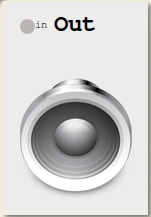
\includegraphics[width=3cm]{../img/png/speaker.png}
\caption{Speaker}
\end{figure}

Ce module vous permet de diriger tout signal fourni en entrée vers la
carte son afin d'entendre le résultat de votre montage.

Notons qu'au plus un Speaker peut-être créé. Essayer d'en faire
apparaître un deuxième est inopérant.

Nous vous mettons en garde contre certains dangers sonores~: produire
des trop basses fréquences (inférieures à 30Hz) avec une forte intensité
peut endommager vos enceintes. Produire des sons trop forts, même sur
une période de courte durée, peut détériorer votre ouïe ainsi que les
rapports que vous entretenez avec vos voisins.
\end{multicols}

\subsection{WAV Looper}

\begin{multicols}{2}
Ce module permet de charger un fichier WAV et de le jouer en boucle,
perpétuellement. Dès l'apparition du WAV Looper sur l'écran, un panneau
s'ouvre et vous propose de charger votre fichier WAV. Attention, seuls
les fichiers WAV au format 44kHz, 16 bits, mono sont autorisés. Si vous
chargez un fichier dans un autre format, aucun son ne sera produit.

Une fois votre fichier chargé, il vous suffit de connecter la sortie
\verb!Out! du module à, par exemple, un Speaker pour entendre votre WAV.
Il vous est également possible de le filtrer grâce à un VCF, comme
n'importe quel signal.

\begin{figure}[H]
\centering
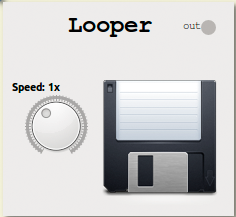
\includegraphics[width=4cm]{../img/png/wavlooper.png}
\caption{WAV Looper}
\end{figure}
\end{multicols}

Une image en forme de disquette est visible~: cliquer dessus vous
permettra de charger un nouveau WAV.

Un potentiomètre \verb!Speed! est disponible~: il permet de modifier la
vitesse de lecture de votre fichier. Par défaut, la vitesse est de 1, ce
qui correspond à la vitesse originale. Une vitesse de 2 provoquera une
lecture deux fois plus rapide, tandis qu'une vitesse de 0.5, deux fois
plus lente.

\subsection{File Output}

\begin{multicols}{2}
\begin{figure}[H]
\centering
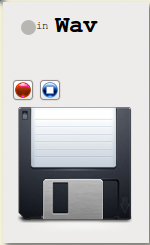
\includegraphics[width=3cm]{../img/png/wavrecorder.png}
\caption{File Output}
\end{figure}

Ce module vous permet d'enregistrer tout signal audio qui serait
connecté à son entrée \verb!In!, vers un fichier WAV. Lors de
l'apparition du module à l'écran, un fenêtre de dialogue vous demande de
choisir le fichier WAV à créer ou remplacer.

Une fois cela fait, il vous
suffit de presser le bouton rouge pour commencer l'enregistrement.
Pressez le bouton \verb!Stop! juste à côté lorsque l'enregistrement est
terminé.

Si vous souhaitez créer un nouvel enregistrement, cliquez de nouveau sur
la disquette afin de choisir un nouveau fichier de destination.

\end{multicols}

\section{Conclusion}

Nous espérons que ce produit vous apportera entière satisfaction.
N'hésitez pas à nous faire part de vos suggestions afin que nous
continuions d'améliorer notre produit~!

\end{document}
